\documentclass{article} % For LaTex2e
\usepackage{iclr2022_conference,times}
% Optional math commands from https://github.com/goodfeli/dlbook_notation.
%%%%% NEW MATH DEFINITIONS %%%%%

\usepackage{amsmath,amsfonts,bm}

% Mark sections of captions for referring to divisions of figures
\newcommand{\figleft}{{\em (Left)}}
\newcommand{\figcenter}{{\em (Center)}}
\newcommand{\figright}{{\em (Right)}}
\newcommand{\figtop}{{\em (Top)}}
\newcommand{\figbottom}{{\em (Bottom)}}
\newcommand{\captiona}{{\em (a)}}
\newcommand{\captionb}{{\em (b)}}
\newcommand{\captionc}{{\em (c)}}
\newcommand{\captiond}{{\em (d)}}

% Highlight a newly defined term
\newcommand{\newterm}[1]{{\bf #1}}


% Figure reference, lower-case.
\def\figref#1{figure~\ref{#1}}
% Figure reference, capital. For start of sentence
\def\Figref#1{Figure~\ref{#1}}
\def\twofigref#1#2{figures \ref{#1} and \ref{#2}}
\def\quadfigref#1#2#3#4{figures \ref{#1}, \ref{#2}, \ref{#3} and \ref{#4}}
% Section reference, lower-case.
\def\secref#1{section~\ref{#1}}
% Section reference, capital.
\def\Secref#1{Section~\ref{#1}}
% Reference to two sections.
\def\twosecrefs#1#2{sections \ref{#1} and \ref{#2}}
% Reference to three sections.
\def\secrefs#1#2#3{sections \ref{#1}, \ref{#2} and \ref{#3}}
% Reference to an equation, lower-case.
\def\eqref#1{equation~\ref{#1}}
% Reference to an equation, upper case
\def\Eqref#1{Equation~\ref{#1}}
% A raw reference to an equation---avoid using if possible
\def\plaineqref#1{\ref{#1}}
% Reference to a chapter, lower-case.
\def\chapref#1{chapter~\ref{#1}}
% Reference to an equation, upper case.
\def\Chapref#1{Chapter~\ref{#1}}
% Reference to a range of chapters
\def\rangechapref#1#2{chapters\ref{#1}--\ref{#2}}
% Reference to an algorithm, lower-case.
\def\algref#1{algorithm~\ref{#1}}
% Reference to an algorithm, upper case.
\def\Algref#1{Algorithm~\ref{#1}}
\def\twoalgref#1#2{algorithms \ref{#1} and \ref{#2}}
\def\Twoalgref#1#2{Algorithms \ref{#1} and \ref{#2}}
% Reference to a part, lower case
\def\partref#1{part~\ref{#1}}
% Reference to a part, upper case
\def\Partref#1{Part~\ref{#1}}
\def\twopartref#1#2{parts \ref{#1} and \ref{#2}}

\def\ceil#1{\lceil #1 \rceil}
\def\floor#1{\lfloor #1 \rfloor}
\def\1{\bm{1}}
\newcommand{\train}{\mathcal{D}}
\newcommand{\valid}{\mathcal{D_{\mathrm{valid}}}}
\newcommand{\test}{\mathcal{D_{\mathrm{test}}}}

\def\eps{{\epsilon}}


% Random variables
\def\reta{{\textnormal{$\eta$}}}
\def\ra{{\textnormal{a}}}
\def\rb{{\textnormal{b}}}
\def\rc{{\textnormal{c}}}
\def\rd{{\textnormal{d}}}
\def\re{{\textnormal{e}}}
\def\rf{{\textnormal{f}}}
\def\rg{{\textnormal{g}}}
\def\rh{{\textnormal{h}}}
\def\ri{{\textnormal{i}}}
\def\rj{{\textnormal{j}}}
\def\rk{{\textnormal{k}}}
\def\rl{{\textnormal{l}}}
% rm is already a command, just don't name any random variables m
\def\rn{{\textnormal{n}}}
\def\ro{{\textnormal{o}}}
\def\rp{{\textnormal{p}}}
\def\rq{{\textnormal{q}}}
\def\rr{{\textnormal{r}}}
\def\rs{{\textnormal{s}}}
\def\rt{{\textnormal{t}}}
\def\ru{{\textnormal{u}}}
\def\rv{{\textnormal{v}}}
\def\rw{{\textnormal{w}}}
\def\rx{{\textnormal{x}}}
\def\ry{{\textnormal{y}}}
\def\rz{{\textnormal{z}}}

% Random vectors
\def\rvepsilon{{\mathbf{\epsilon}}}
\def\rvtheta{{\mathbf{\theta}}}
\def\rva{{\mathbf{a}}}
\def\rvb{{\mathbf{b}}}
\def\rvc{{\mathbf{c}}}
\def\rvd{{\mathbf{d}}}
\def\rve{{\mathbf{e}}}
\def\rvf{{\mathbf{f}}}
\def\rvg{{\mathbf{g}}}
\def\rvh{{\mathbf{h}}}
\def\rvu{{\mathbf{i}}}
\def\rvj{{\mathbf{j}}}
\def\rvk{{\mathbf{k}}}
\def\rvl{{\mathbf{l}}}
\def\rvm{{\mathbf{m}}}
\def\rvn{{\mathbf{n}}}
\def\rvo{{\mathbf{o}}}
\def\rvp{{\mathbf{p}}}
\def\rvq{{\mathbf{q}}}
\def\rvr{{\mathbf{r}}}
\def\rvs{{\mathbf{s}}}
\def\rvt{{\mathbf{t}}}
\def\rvu{{\mathbf{u}}}
\def\rvv{{\mathbf{v}}}
\def\rvw{{\mathbf{w}}}
\def\rvx{{\mathbf{x}}}
\def\rvy{{\mathbf{y}}}
\def\rvz{{\mathbf{z}}}

% Elements of random vectors
\def\erva{{\textnormal{a}}}
\def\ervb{{\textnormal{b}}}
\def\ervc{{\textnormal{c}}}
\def\ervd{{\textnormal{d}}}
\def\erve{{\textnormal{e}}}
\def\ervf{{\textnormal{f}}}
\def\ervg{{\textnormal{g}}}
\def\ervh{{\textnormal{h}}}
\def\ervi{{\textnormal{i}}}
\def\ervj{{\textnormal{j}}}
\def\ervk{{\textnormal{k}}}
\def\ervl{{\textnormal{l}}}
\def\ervm{{\textnormal{m}}}
\def\ervn{{\textnormal{n}}}
\def\ervo{{\textnormal{o}}}
\def\ervp{{\textnormal{p}}}
\def\ervq{{\textnormal{q}}}
\def\ervr{{\textnormal{r}}}
\def\ervs{{\textnormal{s}}}
\def\ervt{{\textnormal{t}}}
\def\ervu{{\textnormal{u}}}
\def\ervv{{\textnormal{v}}}
\def\ervw{{\textnormal{w}}}
\def\ervx{{\textnormal{x}}}
\def\ervy{{\textnormal{y}}}
\def\ervz{{\textnormal{z}}}

% Random matrices
\def\rmA{{\mathbf{A}}}
\def\rmB{{\mathbf{B}}}
\def\rmC{{\mathbf{C}}}
\def\rmD{{\mathbf{D}}}
\def\rmE{{\mathbf{E}}}
\def\rmF{{\mathbf{F}}}
\def\rmG{{\mathbf{G}}}
\def\rmH{{\mathbf{H}}}
\def\rmI{{\mathbf{I}}}
\def\rmJ{{\mathbf{J}}}
\def\rmK{{\mathbf{K}}}
\def\rmL{{\mathbf{L}}}
\def\rmM{{\mathbf{M}}}
\def\rmN{{\mathbf{N}}}
\def\rmO{{\mathbf{O}}}
\def\rmP{{\mathbf{P}}}
\def\rmQ{{\mathbf{Q}}}
\def\rmR{{\mathbf{R}}}
\def\rmS{{\mathbf{S}}}
\def\rmT{{\mathbf{T}}}
\def\rmU{{\mathbf{U}}}
\def\rmV{{\mathbf{V}}}
\def\rmW{{\mathbf{W}}}
\def\rmX{{\mathbf{X}}}
\def\rmY{{\mathbf{Y}}}
\def\rmZ{{\mathbf{Z}}}

% Elements of random matrices
\def\ermA{{\textnormal{A}}}
\def\ermB{{\textnormal{B}}}
\def\ermC{{\textnormal{C}}}
\def\ermD{{\textnormal{D}}}
\def\ermE{{\textnormal{E}}}
\def\ermF{{\textnormal{F}}}
\def\ermG{{\textnormal{G}}}
\def\ermH{{\textnormal{H}}}
\def\ermI{{\textnormal{I}}}
\def\ermJ{{\textnormal{J}}}
\def\ermK{{\textnormal{K}}}
\def\ermL{{\textnormal{L}}}
\def\ermM{{\textnormal{M}}}
\def\ermN{{\textnormal{N}}}
\def\ermO{{\textnormal{O}}}
\def\ermP{{\textnormal{P}}}
\def\ermQ{{\textnormal{Q}}}
\def\ermR{{\textnormal{R}}}
\def\ermS{{\textnormal{S}}}
\def\ermT{{\textnormal{T}}}
\def\ermU{{\textnormal{U}}}
\def\ermV{{\textnormal{V}}}
\def\ermW{{\textnormal{W}}}
\def\ermX{{\textnormal{X}}}
\def\ermY{{\textnormal{Y}}}
\def\ermZ{{\textnormal{Z}}}

% Vectors
\def\vzero{{\bm{0}}}
\def\vone{{\bm{1}}}
\def\vmu{{\bm{\mu}}}
\def\vtheta{{\bm{\theta}}}
\def\va{{\bm{a}}}
\def\vb{{\bm{b}}}
\def\vc{{\bm{c}}}
\def\vd{{\bm{d}}}
\def\ve{{\bm{e}}}
\def\vf{{\bm{f}}}
\def\vg{{\bm{g}}}
\def\vh{{\bm{h}}}
\def\vi{{\bm{i}}}
\def\vj{{\bm{j}}}
\def\vk{{\bm{k}}}
\def\vl{{\bm{l}}}
\def\vm{{\bm{m}}}
\def\vn{{\bm{n}}}
\def\vo{{\bm{o}}}
\def\vp{{\bm{p}}}
\def\vq{{\bm{q}}}
\def\vr{{\bm{r}}}
\def\vs{{\bm{s}}}
\def\vt{{\bm{t}}}
\def\vu{{\bm{u}}}
\def\vv{{\bm{v}}}
\def\vw{{\bm{w}}}
\def\vx{{\bm{x}}}
\def\vy{{\bm{y}}}
\def\vz{{\bm{z}}}

% Elements of vectors
\def\evalpha{{\alpha}}
\def\evbeta{{\beta}}
\def\evepsilon{{\epsilon}}
\def\evlambda{{\lambda}}
\def\evomega{{\omega}}
\def\evmu{{\mu}}
\def\evpsi{{\psi}}
\def\evsigma{{\sigma}}
\def\evtheta{{\theta}}
\def\eva{{a}}
\def\evb{{b}}
\def\evc{{c}}
\def\evd{{d}}
\def\eve{{e}}
\def\evf{{f}}
\def\evg{{g}}
\def\evh{{h}}
\def\evi{{i}}
\def\evj{{j}}
\def\evk{{k}}
\def\evl{{l}}
\def\evm{{m}}
\def\evn{{n}}
\def\evo{{o}}
\def\evp{{p}}
\def\evq{{q}}
\def\evr{{r}}
\def\evs{{s}}
\def\evt{{t}}
\def\evu{{u}}
\def\evv{{v}}
\def\evw{{w}}
\def\evx{{x}}
\def\evy{{y}}
\def\evz{{z}}

% Matrix
\def\mA{{\bm{A}}}
\def\mB{{\bm{B}}}
\def\mC{{\bm{C}}}
\def\mD{{\bm{D}}}
\def\mE{{\bm{E}}}
\def\mF{{\bm{F}}}
\def\mG{{\bm{G}}}
\def\mH{{\bm{H}}}
\def\mI{{\bm{I}}}
\def\mJ{{\bm{J}}}
\def\mK{{\bm{K}}}
\def\mL{{\bm{L}}}
\def\mM{{\bm{M}}}
\def\mN{{\bm{N}}}
\def\mO{{\bm{O}}}
\def\mP{{\bm{P}}}
\def\mQ{{\bm{Q}}}
\def\mR{{\bm{R}}}
\def\mS{{\bm{S}}}
\def\mT{{\bm{T}}}
\def\mU{{\bm{U}}}
\def\mV{{\bm{V}}}
\def\mW{{\bm{W}}}
\def\mX{{\bm{X}}}
\def\mY{{\bm{Y}}}
\def\mZ{{\bm{Z}}}
\def\mBeta{{\bm{\beta}}}
\def\mPhi{{\bm{\Phi}}}
\def\mLambda{{\bm{\Lambda}}}
\def\mSigma{{\bm{\Sigma}}}

% Tensor
\DeclareMathAlphabet{\mathsfit}{\encodingdefault}{\sfdefault}{m}{sl}
\SetMathAlphabet{\mathsfit}{bold}{\encodingdefault}{\sfdefault}{bx}{n}
\newcommand{\tens}[1]{\bm{\mathsfit{#1}}}
\def\tA{{\tens{A}}}
\def\tB{{\tens{B}}}
\def\tC{{\tens{C}}}
\def\tD{{\tens{D}}}
\def\tE{{\tens{E}}}
\def\tF{{\tens{F}}}
\def\tG{{\tens{G}}}
\def\tH{{\tens{H}}}
\def\tI{{\tens{I}}}
\def\tJ{{\tens{J}}}
\def\tK{{\tens{K}}}
\def\tL{{\tens{L}}}
\def\tM{{\tens{M}}}
\def\tN{{\tens{N}}}
\def\tO{{\tens{O}}}
\def\tP{{\tens{P}}}
\def\tQ{{\tens{Q}}}
\def\tR{{\tens{R}}}
\def\tS{{\tens{S}}}
\def\tT{{\tens{T}}}
\def\tU{{\tens{U}}}
\def\tV{{\tens{V}}}
\def\tW{{\tens{W}}}
\def\tX{{\tens{X}}}
\def\tY{{\tens{Y}}}
\def\tZ{{\tens{Z}}}


% Graph
\def\gA{{\mathcal{A}}}
\def\gB{{\mathcal{B}}}
\def\gC{{\mathcal{C}}}
\def\gD{{\mathcal{D}}}
\def\gE{{\mathcal{E}}}
\def\gF{{\mathcal{F}}}
\def\gG{{\mathcal{G}}}
\def\gH{{\mathcal{H}}}
\def\gI{{\mathcal{I}}}
\def\gJ{{\mathcal{J}}}
\def\gK{{\mathcal{K}}}
\def\gL{{\mathcal{L}}}
\def\gM{{\mathcal{M}}}
\def\gN{{\mathcal{N}}}
\def\gO{{\mathcal{O}}}
\def\gP{{\mathcal{P}}}
\def\gQ{{\mathcal{Q}}}
\def\gR{{\mathcal{R}}}
\def\gS{{\mathcal{S}}}
\def\gT{{\mathcal{T}}}
\def\gU{{\mathcal{U}}}
\def\gV{{\mathcal{V}}}
\def\gW{{\mathcal{W}}}
\def\gX{{\mathcal{X}}}
\def\gY{{\mathcal{Y}}}
\def\gZ{{\mathcal{Z}}}

% Sets
\def\sA{{\mathbb{A}}}
\def\sB{{\mathbb{B}}}
\def\sC{{\mathbb{C}}}
\def\sD{{\mathbb{D}}}
% Don't use a set called E, because this would be the same as our symbol
% for expectation.
\def\sF{{\mathbb{F}}}
\def\sG{{\mathbb{G}}}
\def\sH{{\mathbb{H}}}
\def\sI{{\mathbb{I}}}
\def\sJ{{\mathbb{J}}}
\def\sK{{\mathbb{K}}}
\def\sL{{\mathbb{L}}}
\def\sM{{\mathbb{M}}}
\def\sN{{\mathbb{N}}}
\def\sO{{\mathbb{O}}}
\def\sP{{\mathbb{P}}}
\def\sQ{{\mathbb{Q}}}
\def\sR{{\mathbb{R}}}
\def\sS{{\mathbb{S}}}
\def\sT{{\mathbb{T}}}
\def\sU{{\mathbb{U}}}
\def\sV{{\mathbb{V}}}
\def\sW{{\mathbb{W}}}
\def\sX{{\mathbb{X}}}
\def\sY{{\mathbb{Y}}}
\def\sZ{{\mathbb{Z}}}

% Entries of a matrix
\def\emLambda{{\Lambda}}
\def\emA{{A}}
\def\emB{{B}}
\def\emC{{C}}
\def\emD{{D}}
\def\emE{{E}}
\def\emF{{F}}
\def\emG{{G}}
\def\emH{{H}}
\def\emI{{I}}
\def\emJ{{J}}
\def\emK{{K}}
\def\emL{{L}}
\def\emM{{M}}
\def\emN{{N}}
\def\emO{{O}}
\def\emP{{P}}
\def\emQ{{Q}}
\def\emR{{R}}
\def\emS{{S}}
\def\emT{{T}}
\def\emU{{U}}
\def\emV{{V}}
\def\emW{{W}}
\def\emX{{X}}
\def\emY{{Y}}
\def\emZ{{Z}}
\def\emSigma{{\Sigma}}

% entries of a tensor
% Same font as tensor, without \bm wrapper
\newcommand{\etens}[1]{\mathsfit{#1}}
\def\etLambda{{\etens{\Lambda}}}
\def\etA{{\etens{A}}}
\def\etB{{\etens{B}}}
\def\etC{{\etens{C}}}
\def\etD{{\etens{D}}}
\def\etE{{\etens{E}}}
\def\etF{{\etens{F}}}
\def\etG{{\etens{G}}}
\def\etH{{\etens{H}}}
\def\etI{{\etens{I}}}
\def\etJ{{\etens{J}}}
\def\etK{{\etens{K}}}
\def\etL{{\etens{L}}}
\def\etM{{\etens{M}}}
\def\etN{{\etens{N}}}
\def\etO{{\etens{O}}}
\def\etP{{\etens{P}}}
\def\etQ{{\etens{Q}}}
\def\etR{{\etens{R}}}
\def\etS{{\etens{S}}}
\def\etT{{\etens{T}}}
\def\etU{{\etens{U}}}
\def\etV{{\etens{V}}}
\def\etW{{\etens{W}}}
\def\etX{{\etens{X}}}
\def\etY{{\etens{Y}}}
\def\etZ{{\etens{Z}}}

% The true underlying data generating distribution
\newcommand{\pdata}{p_{\rm{data}}}
% The empirical distribution defined by the training set
\newcommand{\ptrain}{\hat{p}_{\rm{data}}}
\newcommand{\Ptrain}{\hat{P}_{\rm{data}}}
% The model distribution
\newcommand{\pmodel}{p_{\rm{model}}}
\newcommand{\Pmodel}{P_{\rm{model}}}
\newcommand{\ptildemodel}{\tilde{p}_{\rm{model}}}
% Stochastic autoencoder distributions
\newcommand{\pencode}{p_{\rm{encoder}}}
\newcommand{\pdecode}{p_{\rm{decoder}}}
\newcommand{\precons}{p_{\rm{reconstruct}}}

\newcommand{\laplace}{\mathrm{Laplace}} % Laplace distribution

\newcommand{\E}{\mathbb{E}}
\newcommand{\Ls}{\mathcal{L}}
\newcommand{\R}{\mathbb{R}}
\newcommand{\emp}{\tilde{p}}
\newcommand{\lr}{\alpha}
\newcommand{\reg}{\lambda}
\newcommand{\rect}{\mathrm{rectifier}}
\newcommand{\softmax}{\mathrm{softmax}}
\newcommand{\sigmoid}{\sigma}
\newcommand{\softplus}{\zeta}
\newcommand{\KL}{D_{\mathrm{KL}}}
\newcommand{\Var}{\mathrm{Var}}
\newcommand{\standarderror}{\mathrm{SE}}
\newcommand{\Cov}{\mathrm{Cov}}
% Wolfram Mathworld says $L^2$ is for function spaces and $\ell^2$ is for vectors
% But then they seem to use $L^2$ for vectors throughout the site, and so does
% wikipedia.
\newcommand{\normlzero}{L^0}
\newcommand{\normlone}{L^1}
\newcommand{\normltwo}{L^2}
\newcommand{\normlp}{L^p}
\newcommand{\normmax}{L^\infty}

\newcommand{\parents}{Pa} % See usage in notation.tex. Chosen to match Daphne's book.

\DeclareMathOperator*{\argmax}{arg\,max}
\DeclareMathOperator*{\argmin}{arg\,min}

\DeclareMathOperator{\sign}{sign}
\DeclareMathOperator{\Tr}{Tr}
\let\ab\allowbreak


%######## APS360: Uncomment your submission name
%\newcommand{\apsname}{Project Proposal}
%\newcommand{\apsname}{Progress Report}
\newcommand{\apsname}{Final Report}

%######## APS360: Put your Group Number here
\newcommand{\gpnumber}{40}

\usepackage{hyperref}
\usepackage{xcolor}
\usepackage[normalem]{ulem}
\usepackage{url}
\usepackage{graphicx}
\usepackage{placeins}
\usepackage{float}

%######## APS360: Put your project Title here
\title{Image Colourization via Convolutional \\
Neural Networks and Deep Learning}

%######## APS360: Put your names, student IDs and Emails here
\author{Youssef Fikry  \\
Student\# 1006682626\\
\texttt{youssef.fikry@mail.utoronto.ca} \\
\And Harkirpa Kaur  \\
Student\# 1011242479 \\
\texttt{harkirpa.kaur@mail.utoronto.ca} \\
\AND
Peter Leong \\
Student\# 1010892955 \\
\texttt{peter.leong@mail.utoronto.ca} \\
\And
Thulasi Thavarajah \\
Student\# 10115358424 \\
\texttt{t.thavarajah@mail.utoronto.ca} \\
\AND
}

% The \author macro works with any number of authors. There are two commands
% used to separate the names and addresses of multiple authors: \And and \AND.
%
% Using \And between authors leaves it to \LaTex{} to determine where to break
% the lines. Using \AND forces a linebreak at that point. So, if \LaTex{}
% puts 3 of 4 authors names on the first line, and the last on the second
% line, try using \AND instead of \And before the third author name.

\newcommand{\fix}{\marginpar{FIx}}
\newcommand{\new}{\marginpar{NEW}}

\iclrfinalcopy 
%######## APS360: Document starts here
\begin{document}


\maketitle

\begin{abstract}
This project addresses the challenge of automated colourization for 256$\times$256 grayscale images using a dataset of 12,600 image pairs, balanced across human subjects, 
animals, and natural scenery. We frame colourization as a supervised learning problem in the CIELAB colour space, where a model predicts chrominance channels ($a^*$, $b^*$) 
from the luminance channel ($L^*$). A shallow convolutional neural network (CNN) provides the baseline performance, while our primary solution employs a deeper convolutional 
encoder-decoder architecture. This design captures high-level semantic features and spatial context, addressing limitations of shallow networks in perceptual realism. All 
source code, datasets, and results are publicly available \href{https://drive.google.com/drive/folders/1cV1NhlQ8UTk_CgJdwhqeRu0z5xE85ZsI?usp=sharing}{here}. 
%######## APS360: Do not change the next line. This shows your Main body page count.
----Total Pages: \pageref{last_page}
\end{abstract}


\section{Introduction}

While colour photography processes first emerged in the 1890s, colour photography did not become widely accessible until the 1970s \citep{scienceandmediamuseum2020}. 
Consequently, most historical photographs remain in black and white, lacking the visual richness that modern viewers are accustomed to. Moreover, individuals who undergo cataract 
removal as part of vision restoration procedures often struggle to interpret grayscale images, rendering many historical photographs inaccessible to them \citet{vogelsang2024impact}. 
This project aims to leverage deep learning to automatically colourize black and white images, with the goal of restoring visual information and improving accessibility for all audiences. 
Traditional, non-deep learning colourization methods tend to produce desaturated results and require extensive human input, limiting their scalability \citep{cheng2016deepcolorization}. 
In contrast, deep neural networks such as convolutional neural networks (CNNs) can effectively learn spatial and semantic features, enabling realistic colourization without user 
intervention \citep{zhang2016colorful}. This makes deep learning a promising and scalable solution for image colourization.

\section{Background \& Related Work}

The challenge of image colourization has been addressed through a range of methods, particularly within deep learning. Even among deep learning-based solutions, researchers 
have proposed a variety of architectures, which can be broadly categorized into five groups: simple colourization neural networks, user-guided colourization networks, diverse 
colourization networks, multi-path networks, and exemplar-based approaches \citep{zeger2021grayscale}.

Simple colourization neural networks use feedforward convolutional neural networks (CNNs) to directly map grayscale inputs to colour outputs. One of the most influential examples 
is the work by \citet{zhang2016colorful}, who proposed a fully convolutional network that predicts the \textit{a} and \textit{b} channels in the CIELAB colour space. Their 
architecture comprises several convolutional layers, each followed by ReLU activations and batch normalization, and is trained as a classification task over quantized ab values, 
producing more vivid outputs than regression-based methods.

User-guided colourization networks incorporate human input to guide the colourization process. \citet{zhang2017real} extended their earlier work by accepting user-provided colour 
“scribbles” as input alongside the grayscale image. The network learns to propagate these hints across the image while minimizing differences from the target colour, allowing 
interactive and controllable colourization.

Diverse colourization networks aim to generate multiple plausible colourizations for a single grayscale input. For instance, \citet{Vitoria2020ChromaGAN} used a generative adversarial 
network (GAN) to produce diverse outputs by learning a conditional distribution over colourizations. This approach addresses the inherent ambiguity in mapping grayscale to colour.

Multi-path colourization networks extract features at multiple spatial resolutions to improve accuracy and context-awareness. \citet{Iizuka2016Colourization} proposed a model with both 
global and local feature pathways, enabling the network to learn both scene-level semantics and fine-grained textures. This structure helps ensure coherent colourization across different 
image regions.

Exemplar-based colourization networks transfer colour information from reference images to the target. In \citet{su2020instanceawareimagecolorization}, instance segmentation is used 
to match regions between the target and exemplars, and two separate colourization networks process this information before merging their outputs. This instance-level guidance simplifies 
the task compared to end-to-end full-image colourization and enhances accuracy in semantically similar scenes.

\section{Data Processing}

 The project's image dataset was compiled using publicly available datasets on Kaggle.com, an online platform that provides access to real-world datasets and a community for data 
 scientists \citep[]{kaggle}. To train a model that can generalize to a broad range of images, the final dataset for this project includes three categories: human, animal, and scenic. 
 All selected datasets are licensed for public domain use. 

\subsection{Repurposing Online Datasets}

The human image dataset, originally intended for human detection, contains a diverse range of 17,300 images of people in different environments \citep[]{kaggle_human}. Furthermore, 
the animal image dataset, initially developed for image classification contains 5,400 images of 90 different animals \citep[]{kaggle_animal}. For this project's purpose, this dataset 
is ideal as it encompasses a diverse set of images with an equal distribution of each animal. Additionally, the scenic image dataset from \citet{kaggle_scene} contains 4,319 images of 
a variety of landscapes spanning a large breadth of colour palettes, potentially influencing the robustness of the final model.

\subsection{Cleaning Up The Datasets}
The team extracted all the images from each dataset and relocated them into folders corresponding to their category (human/animal/scenic). Due to the disparity in the size of the 
three datasets, each dataset was reduced to exactly 4200 images using Python's \verb|random.sample| function with the seed set to 42. The images were then renamed in accordance to 
their respective categories (ex. human\_0001.jpg). 

\begin{figure}[htbp]            % h=here, t=top, b=bottom, p=page float
  \centering
  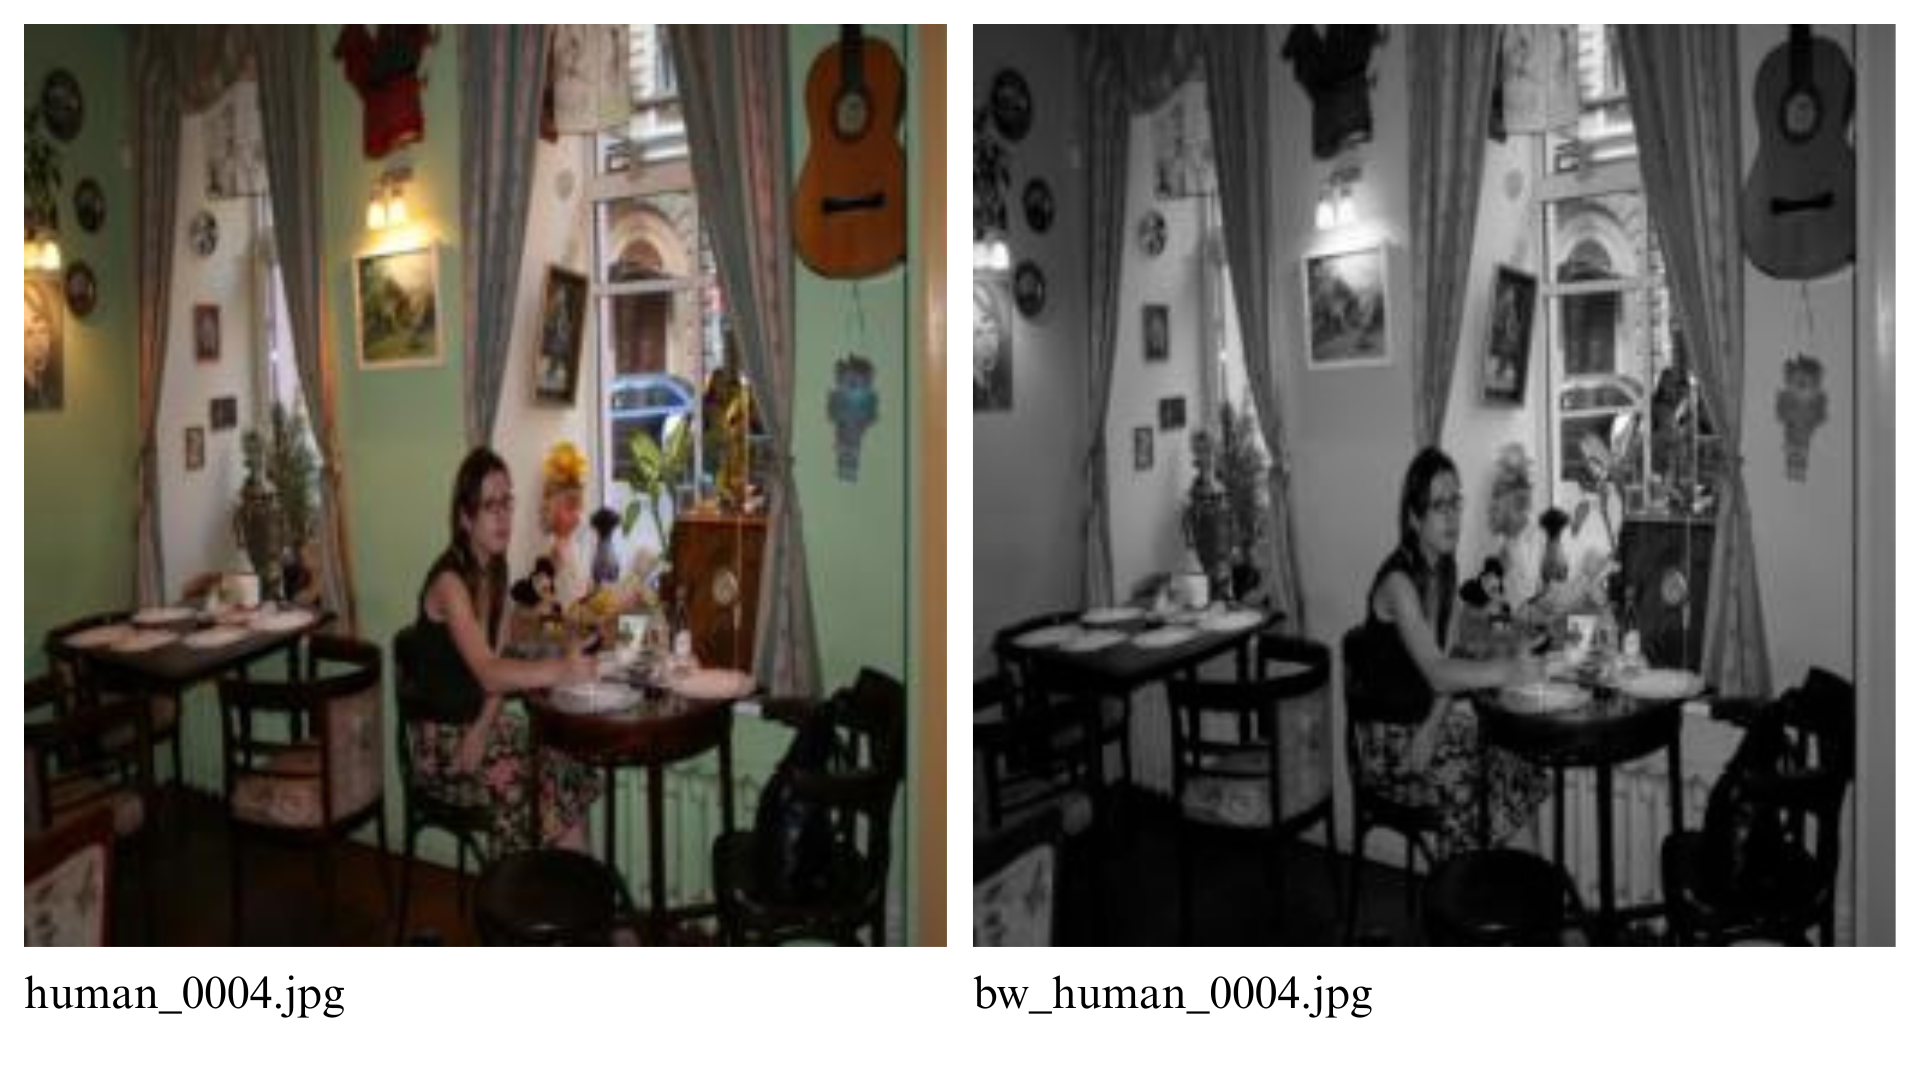
\includegraphics[width=0.65\linewidth]{Figs/Data Example.png}
  \caption{Sample Data Pair from Training Set}
  \label{fig:data_example}
\end{figure}

\subsection{Formatting the Data}

This project requires a unique dataset with black-and-white images paired with their coloured counterparts as the ground truths. To format the cleaned up data and create this dataset, 
PyTorch's \verb|torchvision.transforms| library was utiltized. The team first converted the original images into 256 x 256 pixel ground truth images using the \verb|Resize| transform 
and sorted them according to their category. Following this, \verb|Grayscale| transform with a output channel of 1 was used to convert the 256 x 256 pixel colour images to 256 x 256 
pixel grayscale images to feed into the model. 

\subsection{Splitting Dataset Into Training, Validation and Test Sets}

To create the training, validation and test sets, a ratio of 70:15:15 was chosen. The first 2940 images of each of dataset categories (human/animal/scene) were selected for the training 
set. The remaining images were split evenly to create the validation and testing datasets. 

\subsection{The Final Dataset}

The final dataset is composed of 12,600 pairs of colour and their corresponding grayscale images. Each category (human, animal, and scenic) contains 4,200 image pairs and an even 
distribution of each category was maintained in the training, validation and test sets.

\begin{figure}[htbp]            % h=here, t=top, b=bottom, p=page float
  \centering
  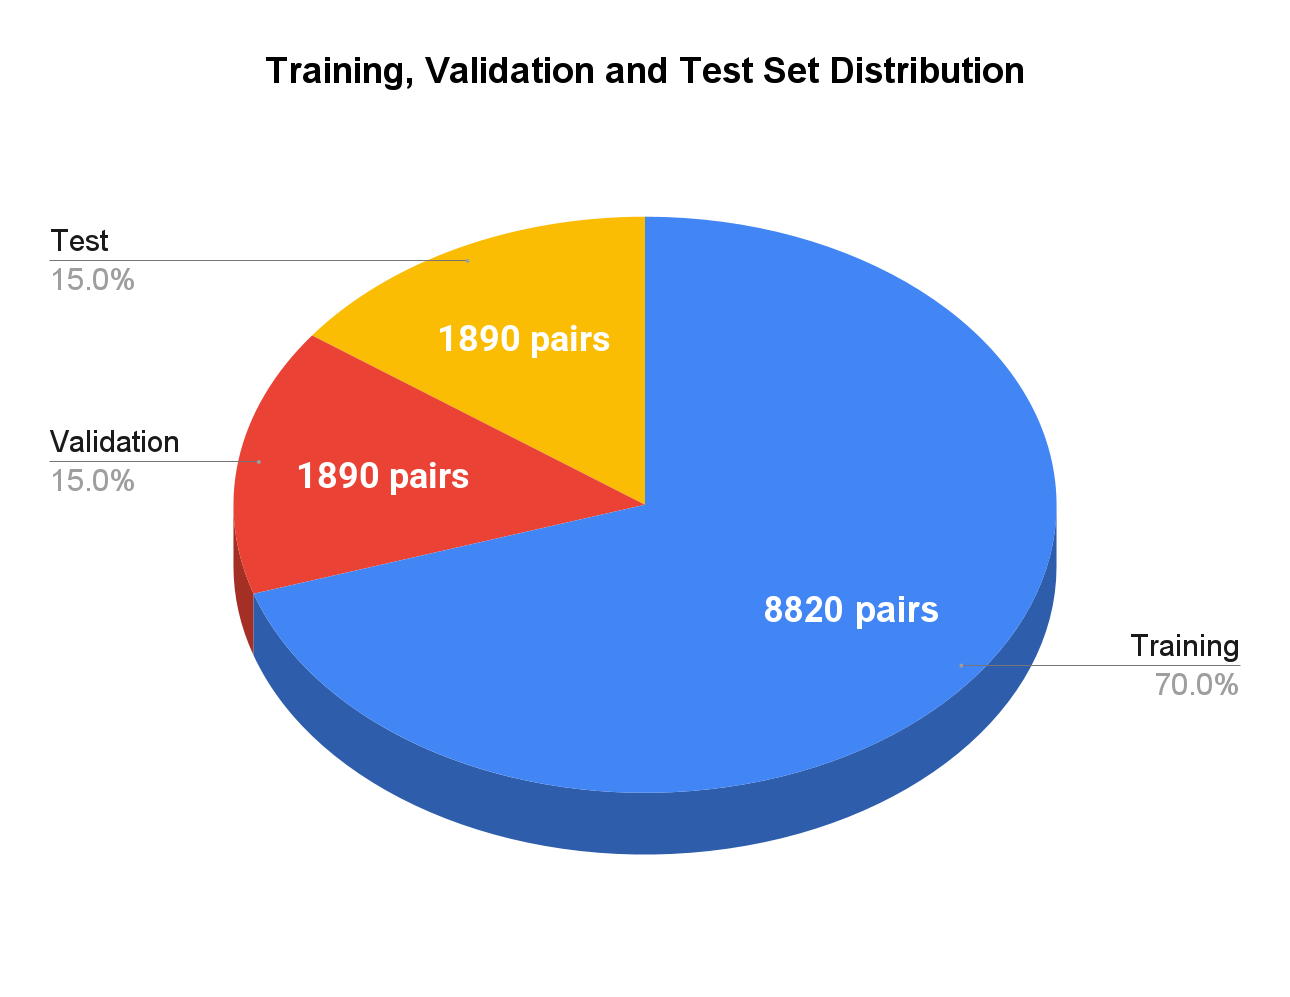
\includegraphics[width=0.65\linewidth]{Figs/dataset1.png}
  \caption{Training, Validation and Test Set Distribution of 12600 Image Pairs}
  \label{fig:dataset}
\end{figure}

\section{Illustration}

\begin{figure}[htbp]            % h=here, t=top, b=bottom, p=page float
  \centering
  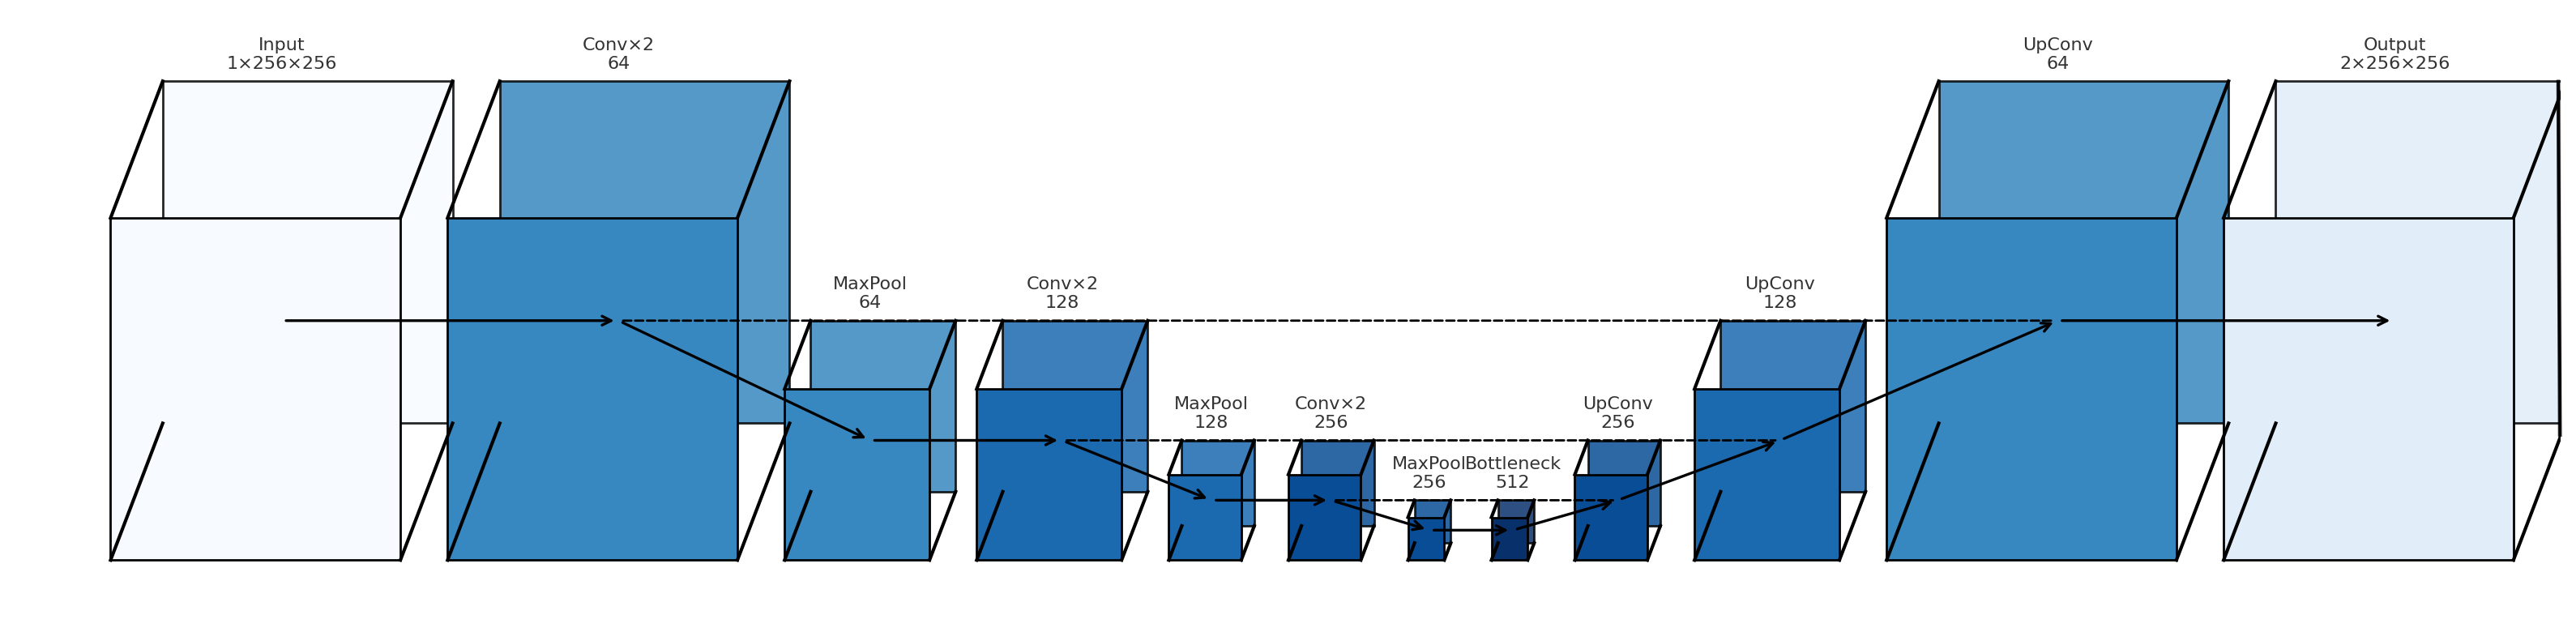
\includegraphics[width=0.9\linewidth]{Figs/architecture.png}
  \caption{Encoder-decoder colourization network with skip connections.}
  \label{fig:architecture}
\end{figure}

The top row shows the encoder, composed of blocks with two convolutional layers followed by max pooling, which progressively downsample the grayscale L channel from 256x256 to 32x32 
while increasing feature depth from 64 to 512. The bottom row depicts the decoder, which uses upsampling blocks to restore full resolution and predict the two chrominance channels 
(a and b). Dashed arrows indicate the three skip connections that transfer fine-grained features from corresponding encoder layers to the decoder stages.

\section{Architecture}

Our primary model for colourization is a convolutional encoder-decoder network, a common architecture for image-to-image translation tasks \citep{leatvanich2025image}. Operating in 
the CIE Lab colour space, the model takes the L channel (lightness) as input and predicts the a and b chrominance channels. To ensure input-target consistency, we derive the L channel 
directly from the same RGB image used to generate the ground truth a,b channels. The predicted chrominance values are then combined with the L channel and converted back to RGB for 
visualization. This use of Lab space decouples intensity from colour, aligning with human perception and typically yielding more realistic results than RGB-based models \citep{leatvanich2025image}.

The architecture resembles a simplified U-Net. The encoder consists of convolutional layers with ReLU activations and batch normalization that progressively downsample the input while 
extracting high-level features. For example, the model starts with a 3×3 convolution producing 64 feature maps, followed by layers with increasing filter counts (e.g., 128), each halving 
spatial resolution. A bottleneck with 256 filters captures abstract representations. The decoder upsamples these back to the original resolution using transposed convolutions, predicting 
the a,b channels. Skip connections between encoder and decoder layers help preserve edge and texture details \citep{leatvanich2025image}.

We initialized the encoder with ResNet-18 weights pretrained on ImageNet, leveraging semantic features learned from large-scale datasets to better infer plausible colours for common 
objects \citep{olah2022lettherebecolor}. The decoder and output layers were trained from scratch.

Rather than formulating colourization as classification over discrete colour bins \citep{olah2022lettherebecolor}, we use a regression-based approach that directly predicts continuous 
a,b values. The model uses a linear output head without tanh activation to avoid chroma saturation and preserve the full colour range.

To encourage vibrant, diverse colourization and reduce bias toward brownish tones, we apply a weighted colour loss informed by a dataset-wide chrominance prior. We also use a robust 
(Huber) pixel loss, which better handles uncertainty and avoids bias toward low-chroma predictions. All augmentations were applied consistently to both input and target images, with 
vertical flips excluded to preserve semantic orientation. Finally, to reduce training time, prior computations were cached and updated once per epoch, reducing training from six hours to one.

\section{Baseline Model}
\label{baseline}

Our main baseline was a shallow encoder-decoder convolutional neural network, designed to be lightweight and fast to train. The model accepted the L channel of a grayscale image as 
input and predicted the a and b chrominance channels. The encoder consisted of two convolutional layers: the first mapped the input to 64 channels using a 3x3 3x3 kernel with padding 1, 
followed by a ReLU activation; the second expanded to 128 channels using the same kernel size and activation. A max pooling layer with a 2x22x2 kernel and stride 2 then reduced the 
spatial resolution by half. This was followed by a bottleneck layer with 256 filters and a ReLU activation, which further processed the compressed feature representation \citep{leatvanich2025image}.

The decoder upsampled the feature map using a transposed convolution that reduced the number of channels from 256 back to 128 while restoring the original resolution, followed by ReLU. 
A final convolutional layer projected to 2 output channels corresponding to the a and b values, and a Tanh activation was applied to constrain the outputs to the normalized Lab colour 
range of [-1,1][-1,1] \citep{rosebrock2019bwcolorization}.

We made no architectural or hyperparameter changes to this baseline throughout the project. It lacked skip connections, pretrained components, or deep 
feature extraction, and as expected, often produced desaturated or muted results. Nonetheless, it served as a clear and reproducible benchmark against which the improvements from our 
full model could be evaluated.

\section{Quantitative Results}
\label{quant_results}

We used a combination of smooth loss and colourfullness metric to calculate the loss values for our model. The colourfullness metric encouraged the model to use more saturated colours
instead of resorting to brown hues, which is an issue we previously encountered. 

Validation and training loss was documented after every epoch and the results were graphed, as shown in Figure~\ref{fig:loss_curve}. We observed some overfitting, as the final training loss was 0.004423, and the final validation loss was 0.007595.

\begin{figure}[htbp]            % h=here, t=top, b=bottom, p=page float
  \centering
  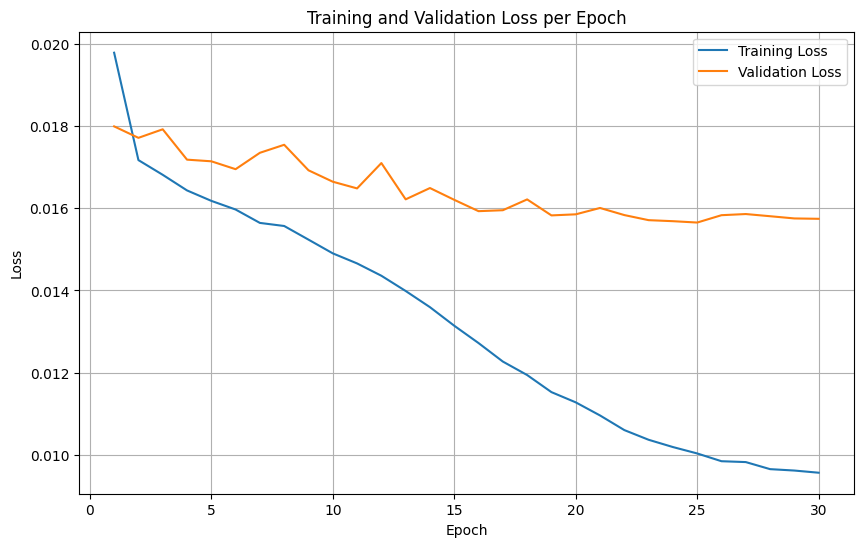
\includegraphics[width=0.9\linewidth]{Figs/loss_curve.png}
  \caption{Learning curve showing training and validation loss of model over 30 epochs.}
  \label{fig:loss_curve}
\end{figure}

\section{Qualitative Results}
\label{qual_results}

Our primary model consistently outperformed the baseline, particularly on landscape scenes where the network was able to recover vibrant skies, foliage, and water with relatively 
realistic hues. In contrast, the baseline produced dull or grayish outputs that lacked semantic colour cues. Figure~\ref{fig:landscape_comparison} shows this clear contrast: while 
the baseline yields low-saturation results, the primary model introduces plausible blue and green tones, suggesting the network successfully learned common associations between luminance 
and scene content.

Performance was less reliable on images of animals and humans, especially when the ground truth involved bright or saturated colours. In these cases, both the baseline and primary models 
tended to favour brownish or muted tones, likely due to the loss function penalizing deviations from average colours. This averaging effect is illustrated in Figure~\ref{fig:final-model-zebra},
where facial features and fur appear washed out or overly neutral.

\begin{figure}[htbp]            % h=here, t=top, b=bottom, p=page float
  \centering
  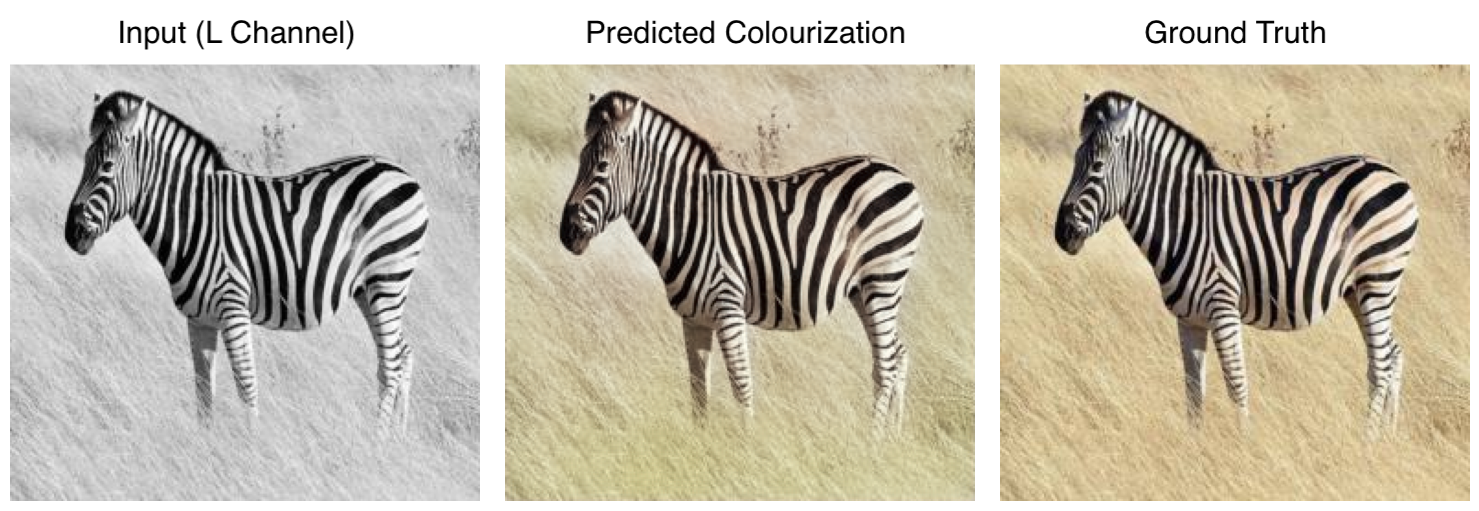
\includegraphics[width=0.9\linewidth]{Figs/final-model-example.png}
  \caption{Example output of a zebra image from the primary model. The model successfully captures the zebra's stripes and fur texture, producing a realistic colourization.}
  \label{fig:final-model-zebra}
\end{figure}

We also experimented with several alternate architectures: diverse colourization, quantized outputs using colour bins, multi-path networks, and exemplar-based models. Despite their 
conceptual appeal, these approaches often underperformed our original model. Figure~\ref{fig:colour-bins-landscape} displays the results from the colour bin model. The exemplar and multi-path models 
frequently introduced a purplish tint across diverse inputs, while the quantized and diverse variants still exhibited the same dulling behaviour due to similar averaging tendencies. 
These results highlight that added architectural complexity does not guarantee improved performance, and in some cases, may exacerbate artefacts or introduce new failure modes.

\begin{figure}[htbp]            % h=here, t=top, b=bottom, p=page float
  \centering
  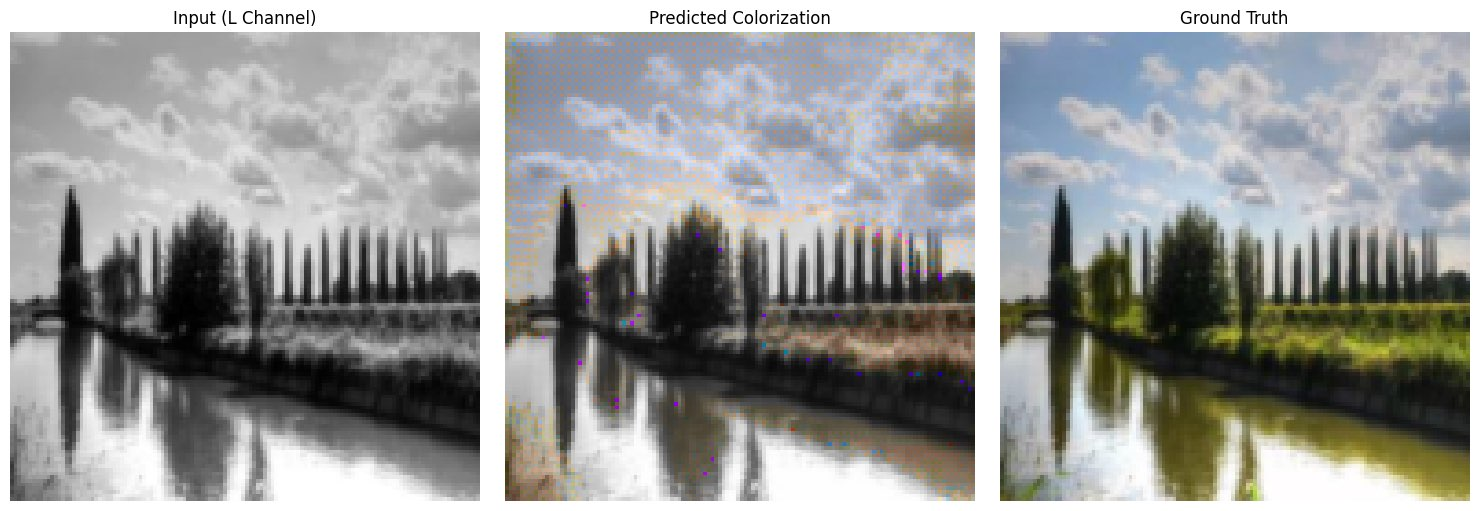
\includegraphics[width=0.9\linewidth]{Figs/colour-bins-landscape.jpg}
  \caption{Example output of the colour bin model on a landscape image. The model attempts to predict colours using quantized bins, but the results are often muted and lack vibrancy.}
  \label{fig:colour-bins-landscape}
\end{figure}

\section{Evaluation on New Data}
\label{new_data}

Our model was evaluated on a separate test set of 1,890 images, which were not used during training or validation. The model performed well relative to the validation results. More explcitly, the model achieved 
a final test loss of 0.007870, which is slightly higher than the validation loss of 0.007595. This indicates that the model generalizes well to unseen data, maintaining its ability to produce realistic colourizations across diverse image categories. 
Included below in \ref{fig:test-data-example} is an example of the model's performance on a test image, demonstrating its ability to capture the scene's structure and colour distribution effectively.

\begin{figure}[htbp]            % h=here, t=top, b=bottom, p=page float
  \centering
  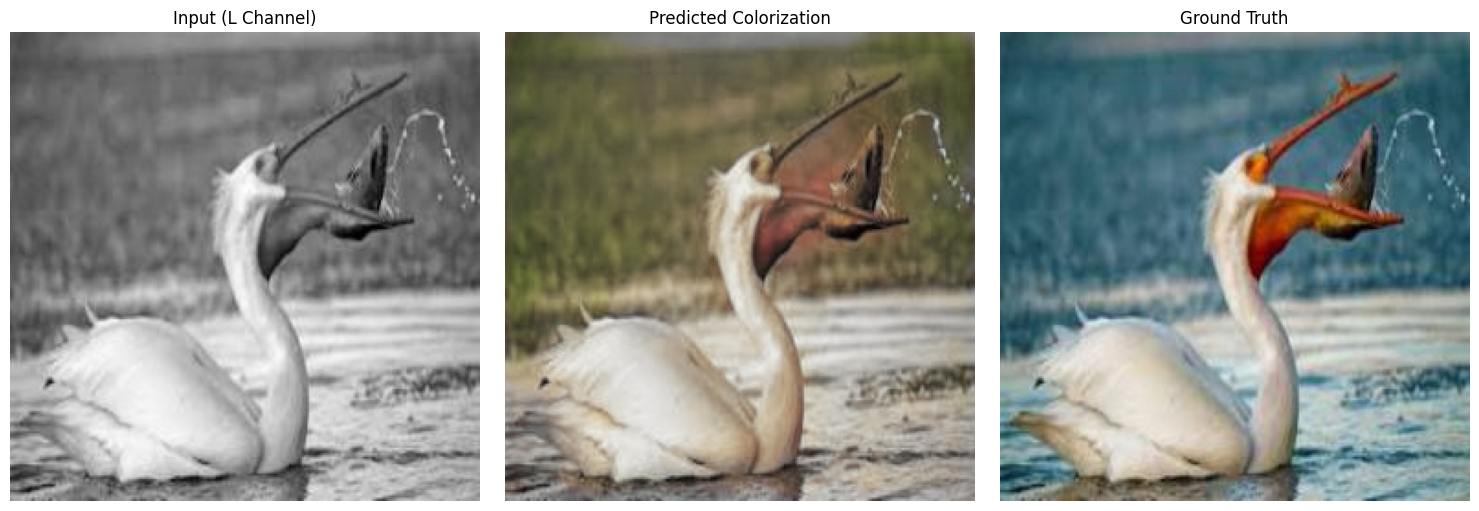
\includegraphics[width=0.9\linewidth]{Figs/test_data_result_example.png}
  \caption{Example output of from the test dataset. The model captures most of the scene's structure and colour distribution, but struggles to produce vibrant blue hues for the water.}
  \label{fig:test-data-example}
\end{figure}

\section{Discussion}
\label{discussion}

Our model generally performed well, especially on landscape images, where predicted colours often aligned well with the ground truth. These results suggest the model successfully
learned broad structural features such as skies, foliage, and terrain. However, performance declined on images featuring humans and animals, particularly when the ground truth
contained highly saturated or vibrant colours. In such cases, both the baseline and our primary model tended toward muted, brownish hues. This behaviour likely arises from the
pixel-wise loss, which encourages the model to average colours to minimize error—resulting in desaturated outputs that reduce loss but compromise visual realism. Furthermore, from colour clustering performed on the dataset (see Figure 7), the most dominant hues were grays and browns; this may have contributed to the preliminary model's muted, brownish outputs. 

\begin{figure}[htbp]            % h=here, t=top, b=bottom, p=page float
  \centering
  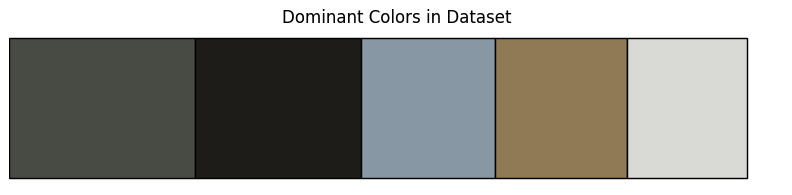
\includegraphics[width=0.95\linewidth]{Figs/dom-colours.png}
  \caption{The dominant five colours in dataset from K-means colour clustering}
  \label{fig:dom-colours}
\end{figure}

To explore alternative strategies, we experimented with several advanced colourization approaches, including diverse colourization (generating multiple plausible outputs),
quantized prediction using discrete colour bins, multi-path architectures, and exemplar-based methods. Despite their conceptual promise, these alternatives failed to outperform
our initial primary model, both quantitatively and qualitatively. In particular, the multi-path and exemplar-based models often produced outputs with a noticeable purple hue, 
suggesting instability or poor alignment between reference features and target content. 
Other approaches encountered similar issues of colour averaging, with results again skewing 
brown or gray to minimize loss.

These findings were unexpected, although the alternative architectures seemed promising in theory, our initial model consistently performed better in both accuracy and visual quality. 
This shows that adding architectural complexity does not necessarily lead to better outcomes. In fact, some modifications introduced new problems—for example, the exemplar-based and 
multi-path models often produced a noticeable purple hue. Others, such as the quantized and diverse models, still struggled with the same tendency to average colours, leading to dull 
or brownish results. Overall, this highlighted the importance of a balanced and well-tuned architecture. Through this process, we learned that effective colourization depends not just 
on network design, but also on careful attention to loss behaviour, data distribution, and how these elements influence model outputs.

\section{Ethical Considerations}
\label{ethical}

The dataset used is publicly available, so there are no copyright or consent concerns. However, there is potential for representation bias, as the dataset may contain imbalances
in race, skin tone, animal breeds, or fur colours. For instance, if lighter-skinned individuals are overrepresented, the model may produce unrealistic or culturally insensitive colourizations 
for darker-skinned individuals. A similar issue applies to animals: limited diversity in breeds or fur patterns may lead to misleading results. While such issues have not visibly appeared in 
our outputs, they remain a risk, especially if colourized images are used for educational purposes or identification tasks.

There is also a risk of evaluation bias. Without knowledge of the dataset's demographic distribution, we cannot ensure the model performs equally well across all categories. This 
uncertainty could skew evaluation metrics and lead to misinterpretation of the model's effectiveness.

Finally, because the model generates plausible but unverifiable outputs, there is a risk that users may place undue trust in the results. It is therefore critical to communicate the model's 
limitations clearly and avoid using it in contexts that require factual accuracy.

\label{last_page}

\newpage
\bibliographystyle{iclr2022_conference}
\bibliography{APS360_Final_Report_ref}


\end{document}
